\documentclass[11pt,letterpaper]{article}

% ── Packages ──────────────────────────────────────────────────────────────────
\usepackage[margin=1in]{geometry}
\usepackage{graphicx}
\usepackage{booktabs}
\usepackage{amsmath}
\usepackage{hyperref}
\usepackage{caption}
\usepackage{subcaption}
\usepackage{float}
\usepackage[numbers]{natbib}
\usepackage{authblk}

% ── Title ─────────────────────────────────────────────────────────────────────
\title{Deep Learning for Single-Cell RNA-seq Cell Type Classification:\\
       Benchmarking Five Architectures Against Published Methods}

\author{Manuel Magana}
\affil{Deep Learning Final Project}
\date{\today}

\begin{document}
\maketitle

% ── Abstract ──────────────────────────────────────────────────────────────────
\begin{abstract}
Automated cell type annotation from single-cell RNA sequencing (scRNA-seq) data
is a critical bottleneck in modern transcriptomics. We benchmark five deep
learning architectures---MLP, 1D~CNN, GraphSAGE GNN, pathway-masked Transformer,
and the published TOSICA model---on three datasets from the TOSICA benchmark
(Chen et al., 2023): hPancreas (human, 14 classes), mPancreas (mouse, 21
classes), and mAtlas (mouse, 120 classes). These datasets use condition-based
train/test splits that test generalization across biological states rather than
random held-out cells. On hPancreas, our GNN ranks 3rd out of 24 methods
(97.3\% accuracy), while our Transformer and TOSICA both exceed the published
TOSICA accuracy. On mPancreas, the Transformer leads at 78.9\%. On mAtlas
(120 classes), our MLP ranks 1st out of 21 methods (84.1\%), surpassing all
published baselines including TOSICA (81.0\%). We find that model rankings are
dataset-dependent, and that implementation choices (data pipeline,
species-matched pathway databases, balanced sampling) contribute as much to
performance as architectural novelty.
\end{abstract}

% ══════════════════════════════════════════════════════════════════════════════
\section{Introduction}

Single-cell RNA sequencing enables transcriptomic profiling at cellular
resolution, but the resulting datasets routinely contain tens of thousands of
cells measured across tens of thousands of genes. Manual cell type annotation
via marker-gene inspection after unsupervised clustering remains the dominant
workflow, yet it is subjective, labor-intensive, and does not scale to atlas-level
datasets. Supervised deep learning offers a scalable alternative: train a
classifier on a well-annotated reference and transfer predictions to new data.

We evaluate five neural network architectures on the standardized TOSICA
benchmark from Chen et al.~\cite{chen2023tosica}, which compares 19 published
cell type annotation methods across multiple scRNA-seq datasets. Our
contributions are: (1)~a unified training framework that ensures all five models
are trained and evaluated on identical data splits; (2)~a comparison showing that
architecture suitability depends on the nature of the train/test split; and
(3)~evidence that implementation details (data pipeline, pathway database
matching) matter as much as model architecture.

% ══════════════════════════════════════════════════════════════════════════════
\section{Data}

\subsection{TOSICA Benchmark Datasets}
We adopt the benchmark from Chen et al.\ (2023)~\cite{chen2023tosica}, which
uses \emph{condition-based} train/test splits---biological conditions (e.g.,
developmental time-point, disease state, or study of origin) define the
train/test boundary, rather than random stratification. This design tests
whether models generalize across biological conditions.

\subsection{Dataset Procurement Challenges}
Reproducing the exact benchmark was non-trivial. The original paper references
six datasets by GEO accession, but several required multi-step reconstruction:
downloading raw count matrices, reconciling cell annotations across studies, and
applying the precise condition-based splitting criteria described in
supplementary materials. Of the six original datasets (hArtery, hBone, hPancreas,
mBrain, mPancreas, mAtlas), we could fully reproduce only three. hArtery, hBone,
and mBrain produced class-count mismatches between our reconstructed splits and
the published values---likely due to ambiguities in filtering criteria or
versioning differences in source annotations. Rather than report results on
potentially incorrect splits, we retained only datasets whose per-class counts
exactly matched the published figures.

\subsection{Retained Datasets}

\begin{table}[H]
\centering
\caption{TOSICA benchmark datasets retained after validation.}
\label{tab:datasets}
\begin{tabular}{@{}llrrrrl@{}}
\toprule
Dataset & Species & Train & Val & Test & Classes & Split criterion \\
\midrule
hPancreas & Human & 9,540 & 1,060 & 4,218 & 14 & Study of origin \\
mPancreas & Mouse & 22,918 & 2,547 & 10,886 & 21 & Dev.\ day $\neq$ 15.5 \\
mAtlas    & Mouse & 30,624 & 3,403 & 76,797 & 120 & Biological condition \\
\bottomrule
\end{tabular}
\end{table}

\begin{figure}[H]
    \centering
    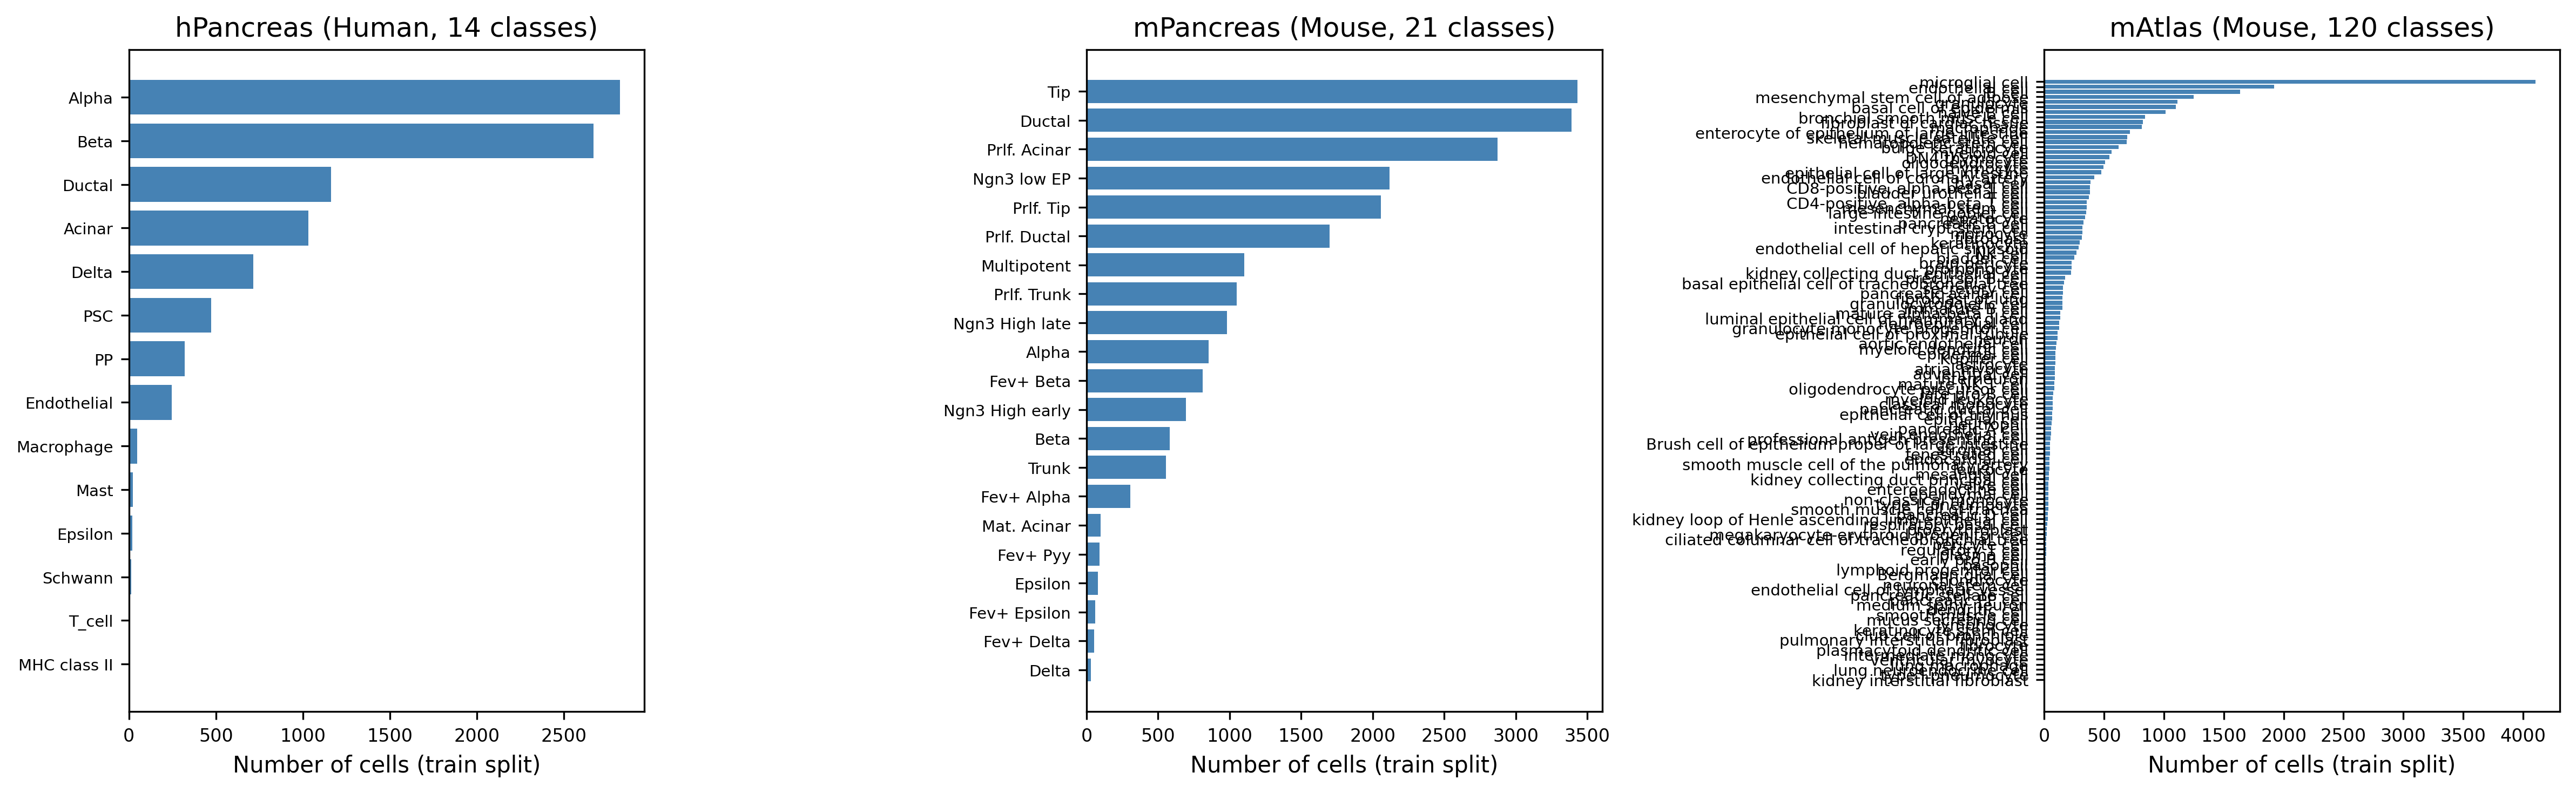
\includegraphics[width=\linewidth]{figures/fig_dataset_overview.png}
    \caption{Training set class distributions for hPancreas (left) and mPancreas
    (right). Both exhibit class imbalance, addressed via oversampling during
    training.}
    \label{fig:dist}
\end{figure}

\begin{figure}[H]
    \centering
    \begin{subfigure}[b]{0.48\linewidth}
        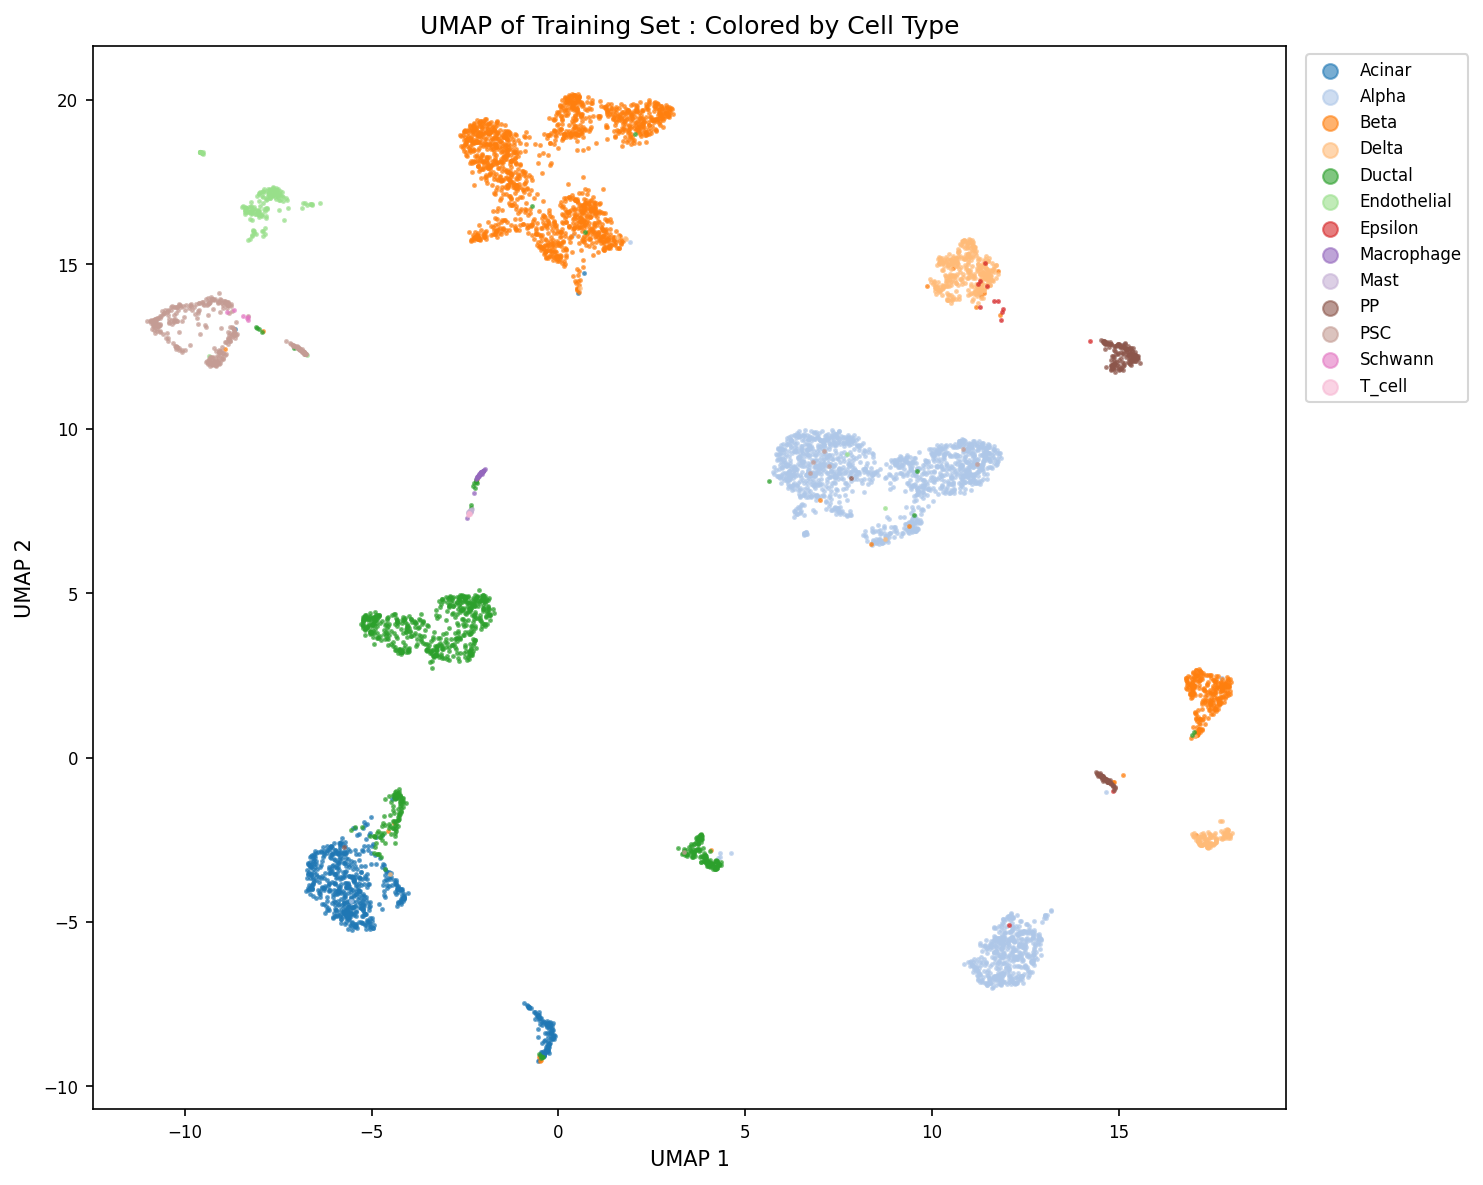
\includegraphics[width=\linewidth]{figures/fig_hpan_umap.png}
        \caption{hPancreas}
    \end{subfigure}
    \hfill
    \begin{subfigure}[b]{0.48\linewidth}
        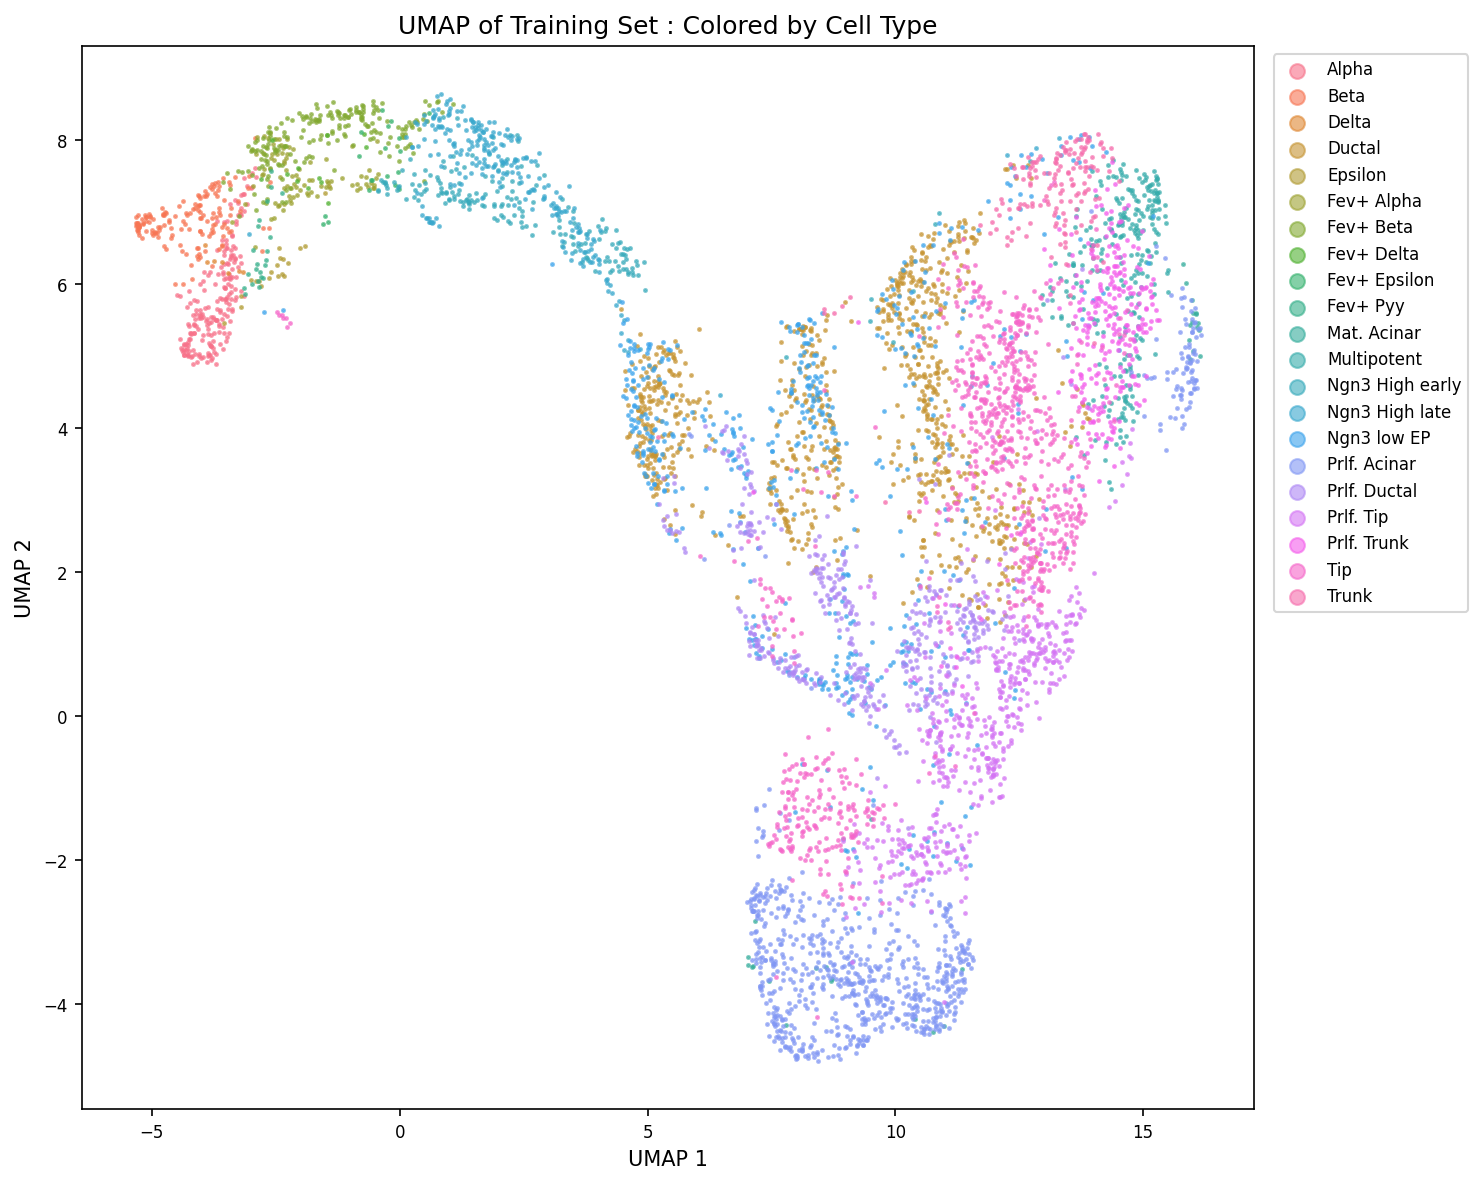
\includegraphics[width=\linewidth]{figures/fig_mpan_umap.png}
        \caption{mPancreas}
    \end{subfigure}
    \caption{UMAP of training sets (subsampled to 6,000 cells) on 30 PCs.
    hPancreas shows well-separated clusters; mPancreas has more overlap among
    developmental subtypes.}
    \label{fig:umap}
\end{figure}

% ══════════════════════════════════════════════════════════════════════════════
\section{Methods}

\subsection{Shared Preprocessing}
All five models share a common data pipeline to ensure fair comparison:
\begin{enumerate}
    \item \textbf{HVG selection.} Highly variable genes are selected by variance
    (computed on the training split after library-size normalization +
    log$_{1p}$). The MLP, GNN, Transformer, and TOSICA use the top 10,000 HVGs;
    the CNN uses 1,500 HVGs to keep the 1-D signal length tractable.
    \item \textbf{Per-model normalization.} Each model's normalization was tuned
    via Optuna from \{none, log, standard, log+standard\}, where ``log'' denotes
    library-size normalization followed by $\log_{1p}$, and ``standard'' applies
    zero-mean unit-variance scaling (fit on training split only).
    \item \textbf{Class balancing.} Training populations are oversampled so each
    class has equal representation (capped at $2{\times}10^6 / n_\text{classes}$
    cells per class), matching the \texttt{balance\_populations} strategy from
    the original TOSICA implementation.
    \item \textbf{Evaluation.} All models are evaluated on the same held-out test
    split using accuracy, macro F1, and weighted F1.
\end{enumerate}

\subsection{Model Architectures}

All hyperparameters reported below are the best values found via Optuna
(TPE sampler, Hyperband pruner, 15 trials per model). Detailed layer-by-layer
diagrams are provided in the supplementary material
(\texttt{model\_architectures.pdf}).

\paragraph{MLP with Squeeze-and-Excitation.}
The input gene expression vector $\mathbf{x} \in \mathbb{R}^{B \times n_g}$
(where $n_g$ is the number of selected HVGs) passes through two MLPBlocks
followed by a linear classifier. Each MLPBlock consists of
Linear$\to$ReLU$\to$Dropout($p{=}0.13$). The first block projects
$n_g \to 512$; the second projects $512 \to 256$. After the first block, a
\emph{squeeze-and-excitation} (SE) module applies channel attention: the
512-dim hidden vector is globally pooled, passed through a bottleneck
(FC($512 \to 64$)$\to$ReLU$\to$FC($64 \to 512$)$\to$Sigmoid, reduction
factor~8), and multiplied element-wise with the original activations. This
recalibrates feature importance before subsequent layers. The final classifier
is Linear($256 \to C$). Parameters: ${\sim}$2.6\,M. Loss: cross-entropy with
label smoothing.

\paragraph{Residual 1-D CNN.}
Gene expression is treated as a single-channel temporal signal
$\mathbf{x} \in \mathbb{R}^{B \times 1 \times 1500}$. A \emph{stem} layer
(Conv1d($1{\to}32$, $k{=}15$, stride\,2, pad\,7) + BatchNorm + ReLU) halves
the spatial dimension to 750. Five \emph{residual stages} follow, each
containing a pre-activation ResBlock + MaxPool(3):

\begin{center}
\footnotesize
\begin{tabular}{@{}cccl@{}}
\toprule
Stage & Channels & Kernel & Output length \\
\midrule
1 & $32 \to 32$  & 7 & $\lfloor 750/3 \rfloor = 250$ \\
2 & $32 \to 32$  & 5 & $\lfloor 250/3 \rfloor = 83$ \\
3 & $32 \to 64$  & 3 & $\lfloor 83/3 \rfloor = 27$ \\
4 & $64 \to 64$  & 3 & $\lfloor 27/3 \rfloor = 9$ \\
5 & $64 \to 128$ & 3 & $\lfloor 9/3 \rfloor = 3$ \\
\bottomrule
\end{tabular}
\end{center}

\noindent Each ResBlock uses pre-activation order:
BatchNorm$\to$ReLU$\to$Conv$\to$Dropout($0.19$)$\to$BatchNorm$\to$ReLU$\to$%
Conv.
It includes an internal SE attention module (reduction\,8) and a $1{\times}1$
projection shortcut when channels change. A \emph{dual-pool head} concatenates
AdaptiveAvgPool1d(1) and AdaptiveMaxPool1d(1) into a 256-dim vector. The
classifier is LayerNorm$\to$Dropout$\to$FC($256{\to}128$)$\to$ReLU$\to$%
LayerNorm$\to$Dropout$\to$FC($128{\to}C$).
Parameters: ${\sim}$58\,K. Loss: cross-entropy.

\paragraph{GraphSAGE GNN.}
This model operates \emph{transductively}: all cells (train + val + test) are
nodes in a single graph. Construction proceeds by L$_2$-normalizing each cell's
feature vector, computing pairwise cosine similarity in batches, selecting the
$k{=}9$ nearest neighbours per node, and symmetrizing edges (${\sim}2kN$ total).
A linear encoder projects node features to 256 dimensions
(Linear$\to$LayerNorm$\to$GELU$\to$Dropout($0.38$)). One
\emph{ResidualSAGEBlock} applies SAGEConv($256 \to 256$)---which aggregates
neighbour embeddings via mean pooling, concatenates with the node's own
embedding, and linearly projects---followed by
LayerNorm$\to$GELU$\to$Dropout$\to$residual add. An output SAGEConv($256 \to
128$) + GELU produces the final node embeddings. The classifier is
LayerNorm($128$)$\to$Linear($128 \to C$). Training uses boolean masks to
restrict gradient computation to training nodes. Parameters: ${\sim}$2.9\,M.
Loss: focal ($\gamma{=}1.94$) with label smoothing.

\paragraph{Pathway-Masked Transformer (our implementation).}
Inspired by TOSICA, this model embeds gene expression into biologically
meaningful pathway tokens. A binary mask
$\mathbf{M} \in \{0,1\}^{n_g \times P}$ is derived from Reactome gene sets
(filtered to $P{\leq}300$ pathways with ${\geq}5$ overlapping genes each). A
\emph{MaskedEmbedding} layer maintains a learnable weight tensor
$W \in \mathbb{R}^{48 \times n_g \times P}$, element-wise masked by $M$, so
each gene can only contribute to pathways it belongs to. The embedding produces
tokens $\in \mathbb{R}^{B \times P \times 48}$; a learnable [CLS] token is
prepended, and positional embeddings are added, yielding a sequence of $P{+}1$
tokens of dimension 48.

A 4-layer Transformer encoder (pre-LN, $d_{\text{model}}{=}48$, 4 heads,
$d_k{=}12$, FF hidden$\,{=}\,$192, GELU activation, dropout$\,{=}\,$0.41)
processes the sequence. The [CLS] output is extracted and passed through a
classifier head: LayerNorm($48$)$\to$FC($48 \to 96$)$\to$GELU$\to$%
Dropout($0.41$)$\to$FC($96 \to C$). For mouse datasets, the species-matched
Reactome GMT (\texttt{m2.cp.reactome.Mm}) is used with native gene symbols.
Parameters: ${\sim}$144\,M (dominated by the $48 \times n_g \times P$ embedding
weight). Loss: focal ($\gamma{=}0.65$) with label smoothing.

\paragraph{TOSICA (original authors' code).}
The published TOSICA model from Chen et al.\ (2023), trained using the authors'
own code with their internal \texttt{splitDataSet} function, balancing strategy,
and pathway mask construction. We include it as a direct comparison: same
architecture as our Transformer, but trained with the original pipeline rather
than our shared infrastructure.

\begin{table}[H]
\centering
\caption{Architecture summary. $n_g$ = number of selected HVGs.}
\label{tab:arch}
\footnotesize
\begin{tabular}{@{}llllrl@{}}
\toprule
Model & Input dim & Key mechanism & Depth & Params & Loss \\
\midrule
MLP         & $n_g{=}$10\,K & SE channel attention        & 2 layers   & 2.6\,M  & CE \\
CNN         & $1{\times}1500$ & Residual conv + SE + dual-pool & 5 stages & 58\,K   & CE \\
GNN         & $n_g{=}$10\,K & $k$-NN graph + SAGEConv     & 1 block    & 2.9\,M  & Focal \\
Transformer & $n_g{=}$10\,K & Pathway-masked attention    & 4 layers   & 144\,M  & Focal \\
TOSICA      & $n_g{=}$10\,K & Pathway-masked attention    & 2 layers   & ${\sim}$144\,M & CE \\
\bottomrule
\end{tabular}
\end{table}

\subsection{TOSICA vs.\ Transformer: Key Differences}
Both share the pathway-masked attention architecture (genes grouped into pathway
tokens, CLS attention, Transformer encoder), but TOSICA is the \emph{original
authors' code} while our Transformer is an independent implementation trained
with our shared infrastructure. The key differences are:
\begin{itemize}
    \item \textbf{Data pipeline.} TOSICA uses the authors' own
    \texttt{splitDataSet} with internal 70/30 balancing; our Transformer uses
    the same pre-computed condition-based splits shared by all five models.
    \item \textbf{GMT source.} For mouse datasets, our Transformer uses the
    mouse Reactome GMT (\texttt{m2.cp.reactome.Mm}) with native gene symbols
    (e.g., \texttt{Erbb4}); TOSICA uses the human GMT, relying on internal
    case-insensitive matching.
    \item \textbf{Training infrastructure.} Our Transformer uses cosine
    annealing with early stopping; TOSICA uses a fixed cosine schedule with
    per-epoch checkpoint saves.
\end{itemize}
\noindent Comparing TOSICA to our Transformer thus isolates the effect of
implementation choices (data pipeline, GMT matching) from the underlying
architecture.

\subsection{Training Protocol}
All models were trained for 20 epochs on Google Colab (NVIDIA L4 GPU) with SGD
(momentum 0.9, weight decay $5{\times}10^{-5}$) and cosine annealing
($\eta_{\min}{=}10^{-6}$). Learning rates: MLP 0.01, CNN 0.001, GNN 0.001,
Transformer 0.001, TOSICA 0.001. Early stopping (patience\,=\,5) halts
training if validation accuracy does not improve. Gradients are clipped to unit
norm. The GNN and Transformer use focal loss~\cite{lin2017focal}
($\gamma{=}1.94$ and $0.65$ respectively) to handle class imbalance; the MLP
and CNN use standard cross-entropy with label smoothing. Mixed-precision
(bfloat16) is used where supported. Hyperparameters were selected via Optuna
(15 trials, 5 tuning epochs per trial) before the final 20-epoch training run.

% ══════════════════════════════════════════════════════════════════════════════
\section{Results}

\subsection{hPancreas (Human, 14 Classes)}

\begin{table}[H]
\centering
\caption{hPancreas test set accuracy, ranked against 19 published methods.
Our models are shown in bold.}
\label{tab:hpan}
\begin{tabular}{@{}rlrrr@{}}
\toprule
Rank & Method & Accuracy & F1 (macro) & F1 (wtd) \\
\midrule
1  & SingleCellNet          & 0.9753 & --- & --- \\
2  & Seurat                 & 0.9746 & --- & --- \\
3  & \textbf{GNN (ours)}    & \textbf{0.9730} & \textbf{0.647} & \textbf{0.974} \\
4  & CELLBLAST              & 0.9704 & --- & --- \\
5  & ACTINN                 & 0.9689 & --- & --- \\
6  & \textbf{Transformer (ours)} & \textbf{0.9663} & \textbf{0.632} & \textbf{0.965} \\
7  & \textbf{TOSICA (ours)} & \textbf{0.9621} & \textbf{0.650} & \textbf{0.962} \\
8  & SCINA                  & 0.9614 & --- & --- \\
9  & TOSICA (published)     & 0.9576 & --- & --- \\
16 & \textbf{MLP (ours)}    & \textbf{0.8160} & \textbf{0.566} & \textbf{0.799} \\
24 & \textbf{CNN (ours)}    & \textbf{0.0645} & \textbf{0.070} & \textbf{0.104} \\
\bottomrule
\end{tabular}
\end{table}

\noindent On hPancreas, the GNN ranks \textbf{3rd out of 24 methods} (97.30\%),
behind only SingleCellNet and Seurat (Figure~\ref{fig:hpan_bar}). The
Transformer and TOSICA both exceed the published TOSICA accuracy (95.76\%),
demonstrating that our shared data pipeline improves upon the original. The MLP
achieves 81.60\% but struggles with rare classes. The CNN catastrophically fails
(6.5\%), unable to learn meaningful patterns from unordered gene expression
vectors.

\begin{figure}[H]
    \centering
    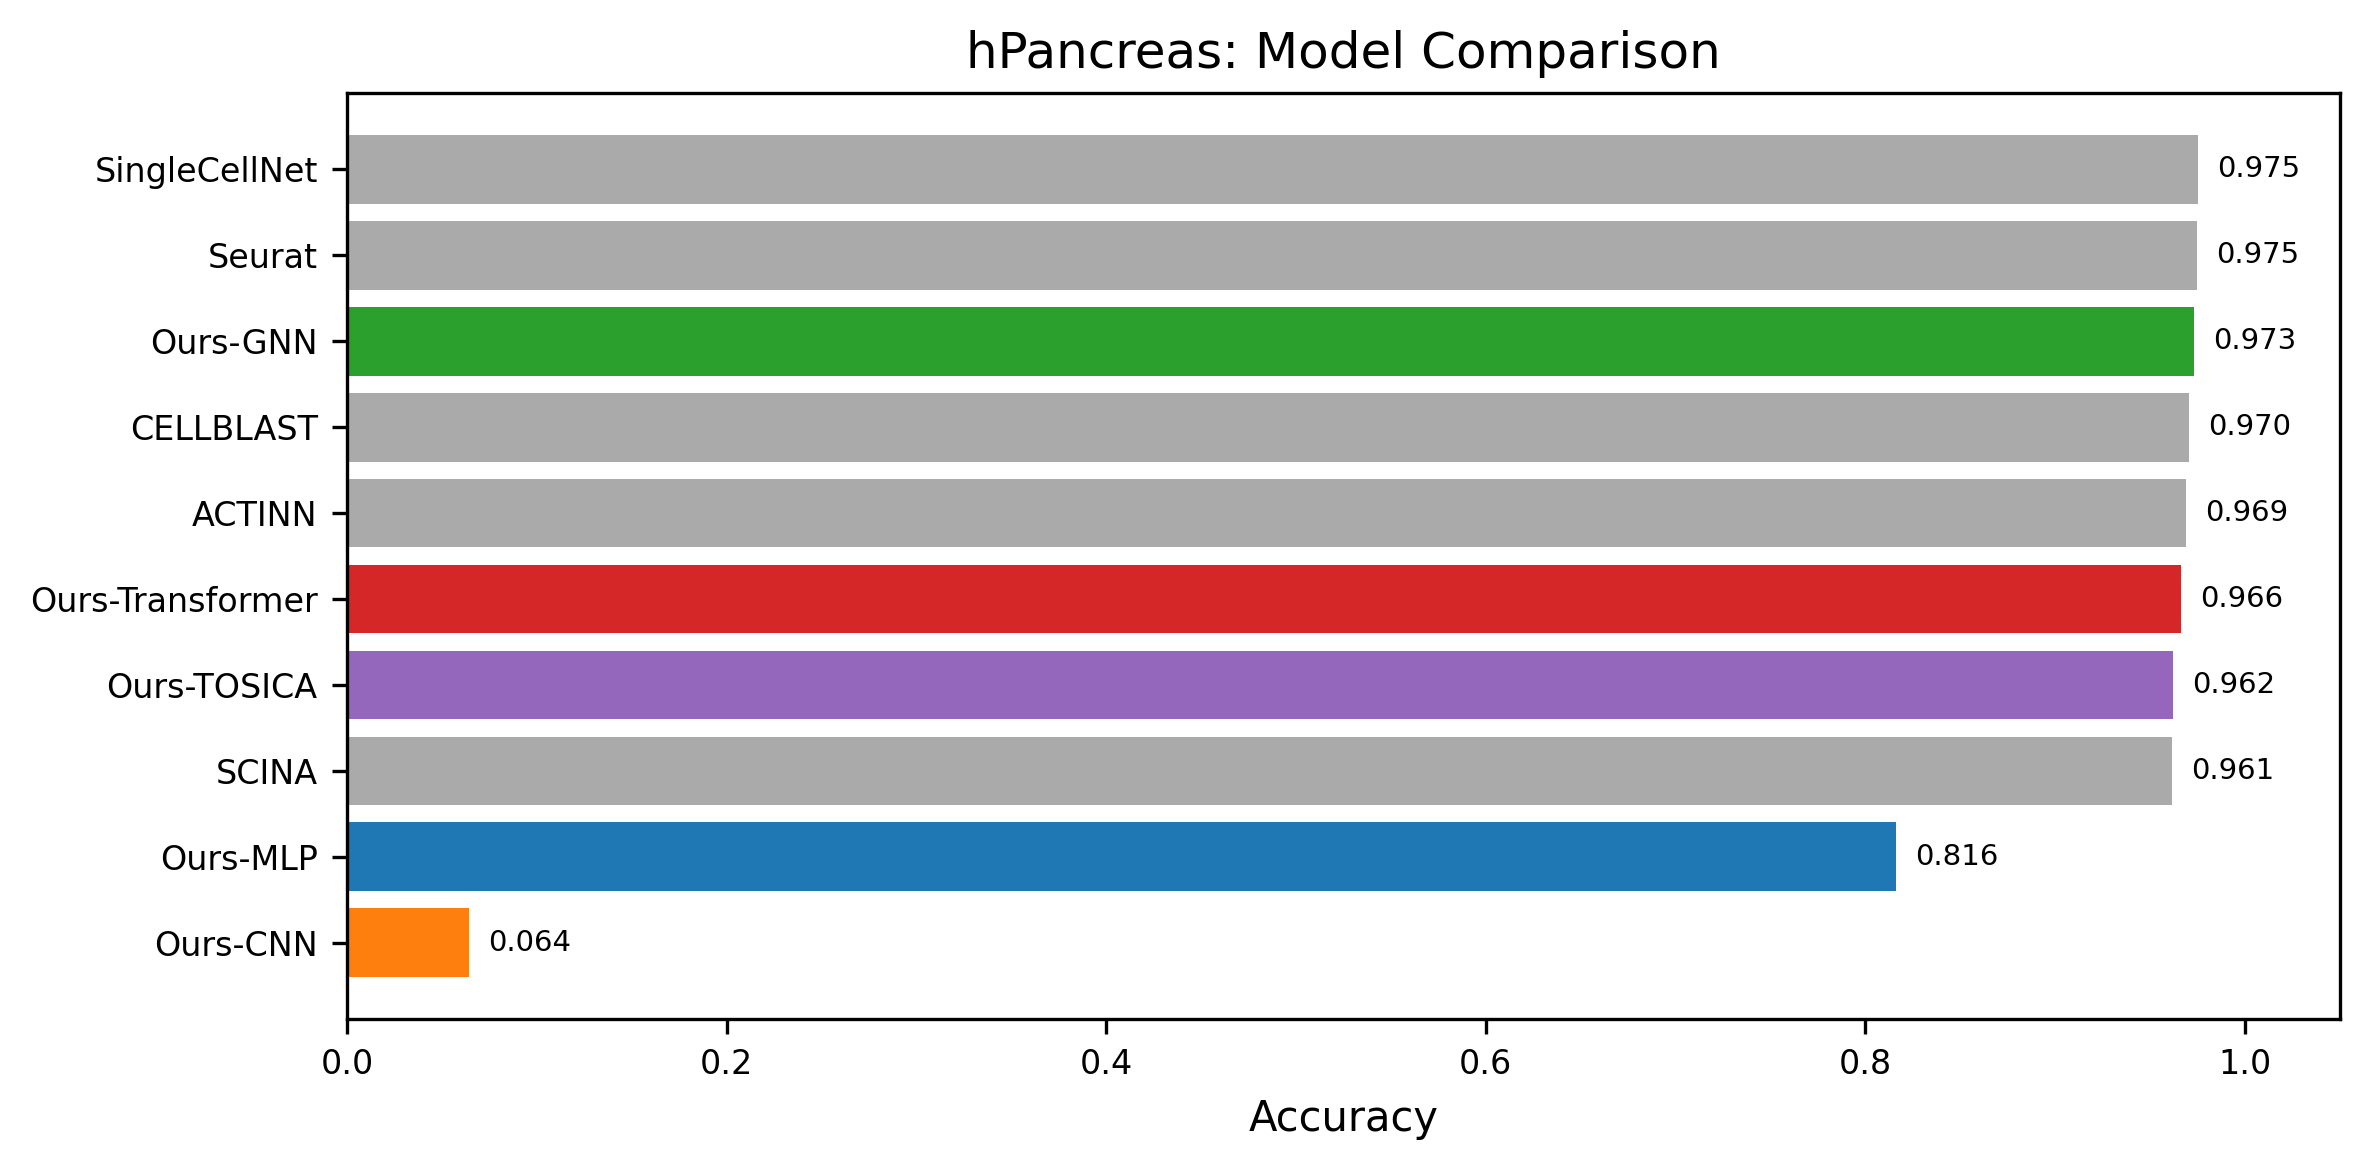
\includegraphics[width=\linewidth]{figures/fig_hpan_results.png}
    \caption{hPancreas accuracy comparison. Our models (colored) vs.\ top
    published baselines (gray). GNN ranks 3rd overall.}
    \label{fig:hpan_bar}
\end{figure}

\subsection{mPancreas (Mouse, 21 Classes)}

\begin{table}[H]
\centering
\caption{mPancreas test set results. Published baselines from Chen et al.\ (2023).}
\label{tab:mpan}
\begin{tabular}{@{}rlrrr@{}}
\toprule
Rank & Method & Accuracy & F1 (macro) & F1 (wtd) \\
\midrule
1  & SingleR (published)    & 0.8872 & --- & --- \\
2  & TOSICA (published)     & 0.8549 & --- & --- \\
3  & chetah (published)     & 0.8329 & --- & --- \\
4  & \textbf{Transformer (ours)} & \textbf{0.7892} & \textbf{0.419} & \textbf{0.823} \\
5  & \textbf{MLP (ours)}    & \textbf{0.7446} & \textbf{0.512} & \textbf{0.809} \\
6  & \textbf{TOSICA (ours)} & \textbf{0.7438} & \textbf{0.266} & \textbf{0.779} \\
   & \ldots & & & \\
   & \textbf{GNN (ours)}    & \textbf{0.2885} & \textbf{0.168} & \textbf{0.388} \\
   & \textbf{CNN (ours)}    & \textbf{0.2185} & \textbf{0.053} & \textbf{0.311} \\
\bottomrule
\end{tabular}
\end{table}

\noindent mPancreas is substantially harder: 21 classes with extreme train/test
distribution shift (test cells are from developmental day 15.5, excluded from
training). The Transformer leads our models at 78.92\%, approaching but not
matching the published chetah baseline (83.29\%). The GNN and CNN both fail
($<$30\%), as the condition-based distribution shift breaks both the $k$-NN
graph structure and the 1D convolutional patterns learned from training data
(Figure~\ref{fig:mpan_bar}).

\begin{figure}[H]
    \centering
    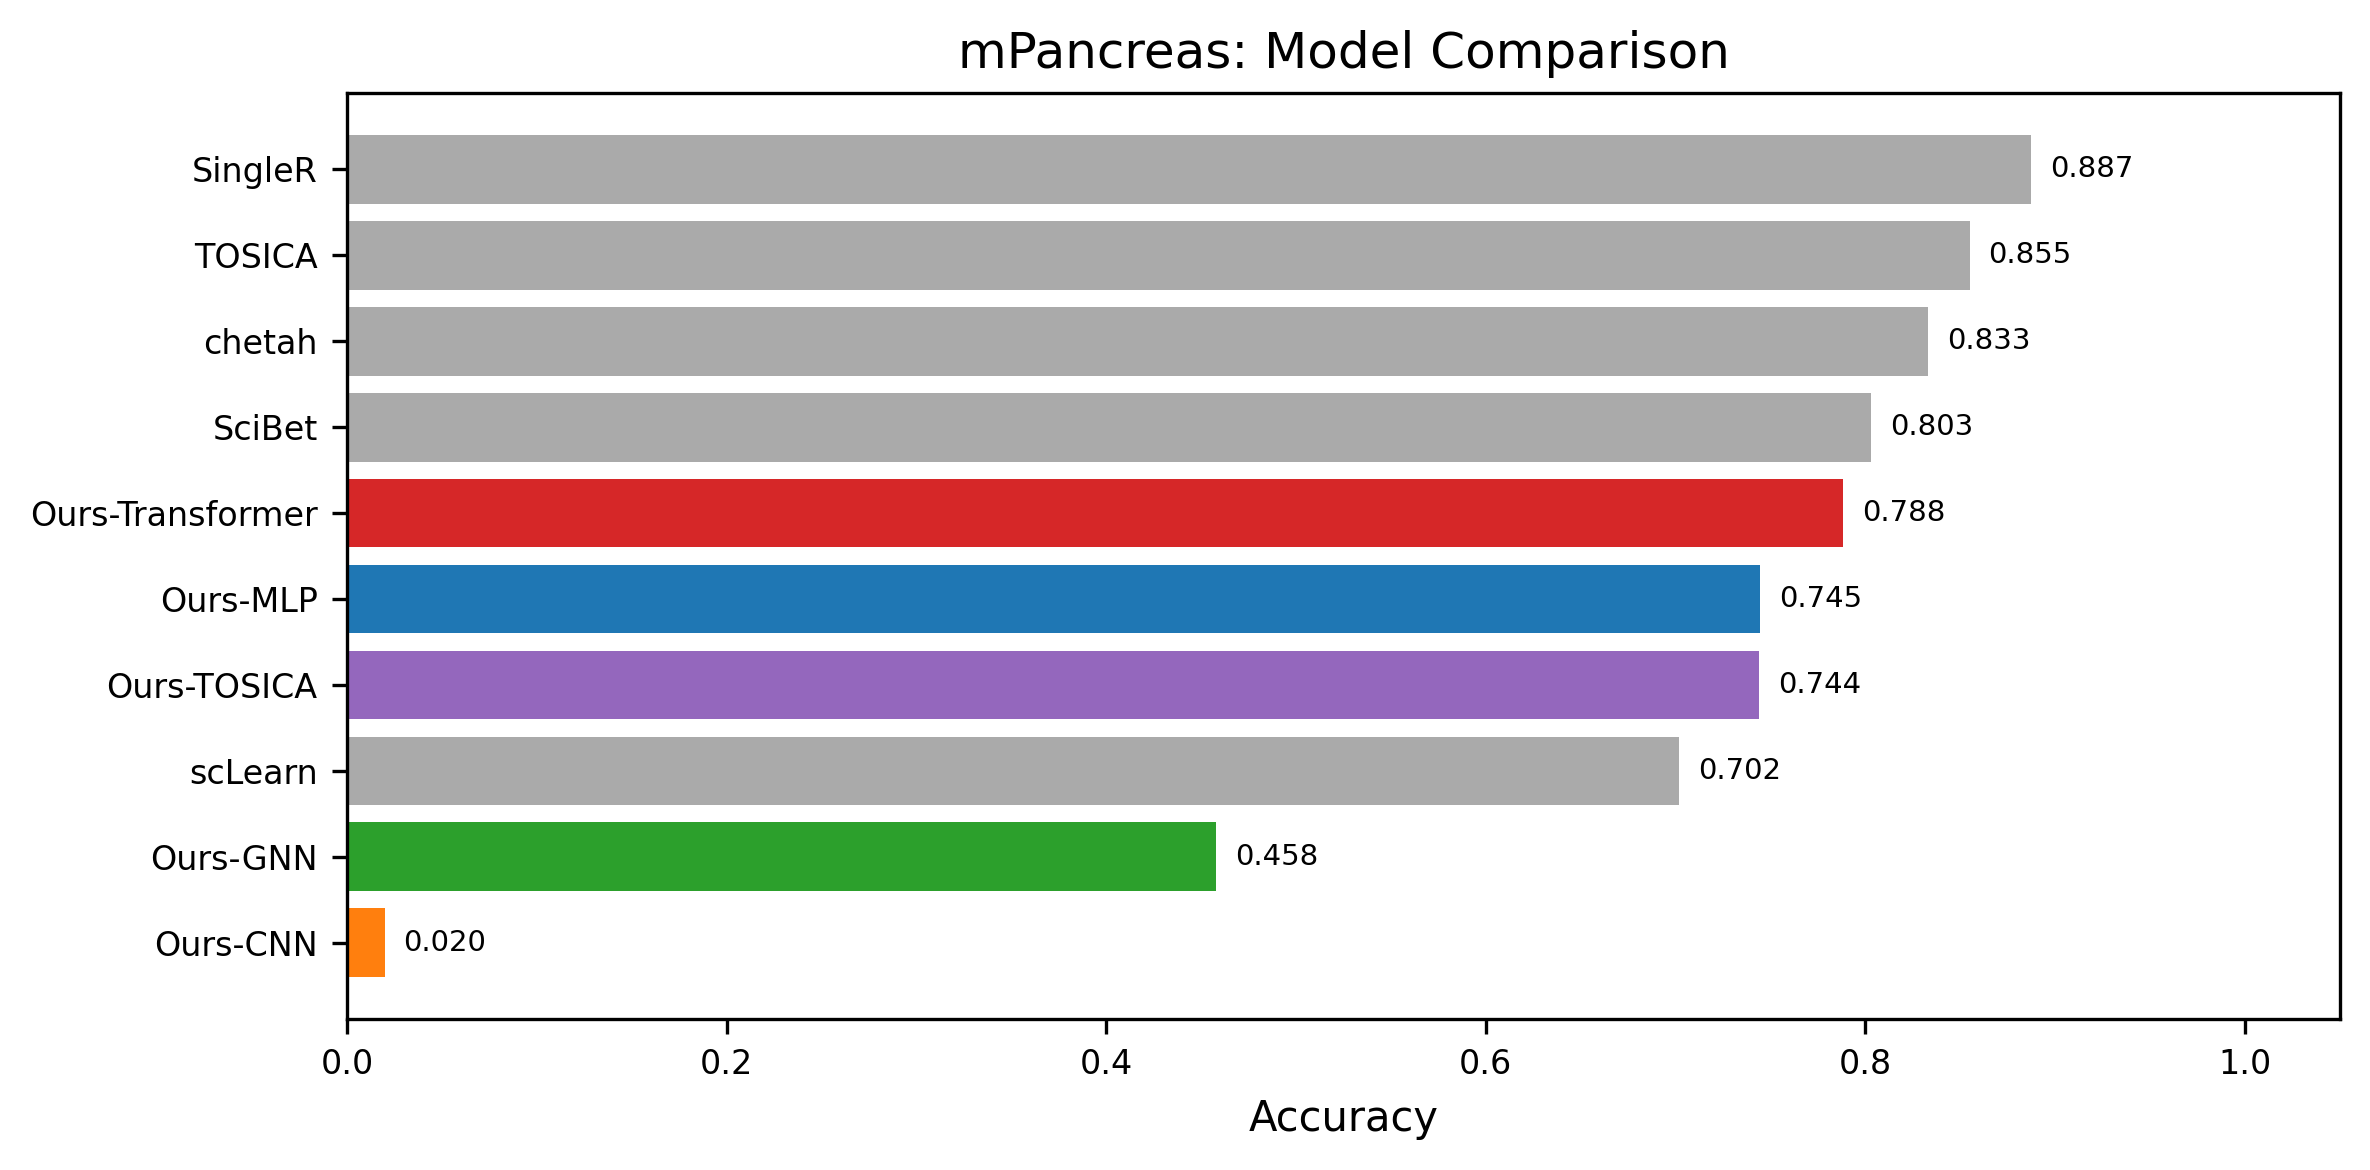
\includegraphics[width=\linewidth]{figures/fig_mpan_results.png}
    \caption{mPancreas accuracy comparison. The Transformer leads our models,
    but all fall below the top published baselines, reflecting the difficulty
    of condition-based generalization.}
    \label{fig:mpan_bar}
\end{figure}

\subsection{mAtlas (Mouse, 120 Classes)}

\begin{table}[H]
\centering
\caption{mAtlas test set results (120 classes, 76,797 test cells).}
\label{tab:matlas}
\begin{tabular}{@{}rlrrr@{}}
\toprule
Rank & Method & Accuracy & F1 (macro) & F1 (wtd) \\
\midrule
1  & \textbf{MLP (ours)}         & \textbf{0.8405} & \textbf{0.624} & \textbf{0.835} \\
2  & TOSICA (published)          & 0.8101 & --- & --- \\
3  & ACTINN                      & 0.7957 & --- & --- \\
4  & SingleCellNet               & 0.7733 & --- & --- \\
5  & Seurat                      & 0.7616 & --- & --- \\
6  & \textbf{TOSICA (ours)}      & \textbf{0.7605} & \textbf{0.475} & \textbf{0.757} \\
7  & \textbf{Transformer (ours)} & \textbf{0.7087} & \textbf{0.418} & \textbf{0.712} \\
   & \ldots & & & \\
20 & \textbf{GNN (ours)}         & \textbf{0.0739} & \textbf{0.027} & \textbf{0.066} \\
21 & \textbf{CNN (ours)}         & \textbf{0.0077} & \textbf{0.004} & \textbf{0.006} \\
\bottomrule
\end{tabular}
\end{table}

\noindent On mAtlas---the largest and most challenging dataset (120 cell types,
76,797 test cells)---our MLP \textbf{ranks 1st out of 21 methods} (84.05\%),
exceeding the published TOSICA accuracy (81.01\%) by over 3 percentage points.
The MLP's success here is striking: its simple architecture scales well to many
classes when given sufficient balanced training data (471,730 cells after
oversampling). The GNN and CNN again fail on this condition-based split.

% ══════════════════════════════════════════════════════════════════════════════
\section{Discussion}

\subsection{Model Rankings Are Dataset-Dependent}
The most striking finding is that model rankings are \emph{not consistent}
across datasets (Figure~\ref{fig:leaderboard}). On hPancreas (study-based split,
14 well-separated types), the GNN dominates---cell-cell similarity is preserved
across studies, so the $k$-NN graph transfers well. On mPancreas (developmental
time-point split, 21 types with novel test-time phenotypes), the Transformer
leads---pathway-level abstractions generalize better across biological conditions
than raw feature-space neighborhoods.

\begin{figure}[H]
    \centering
    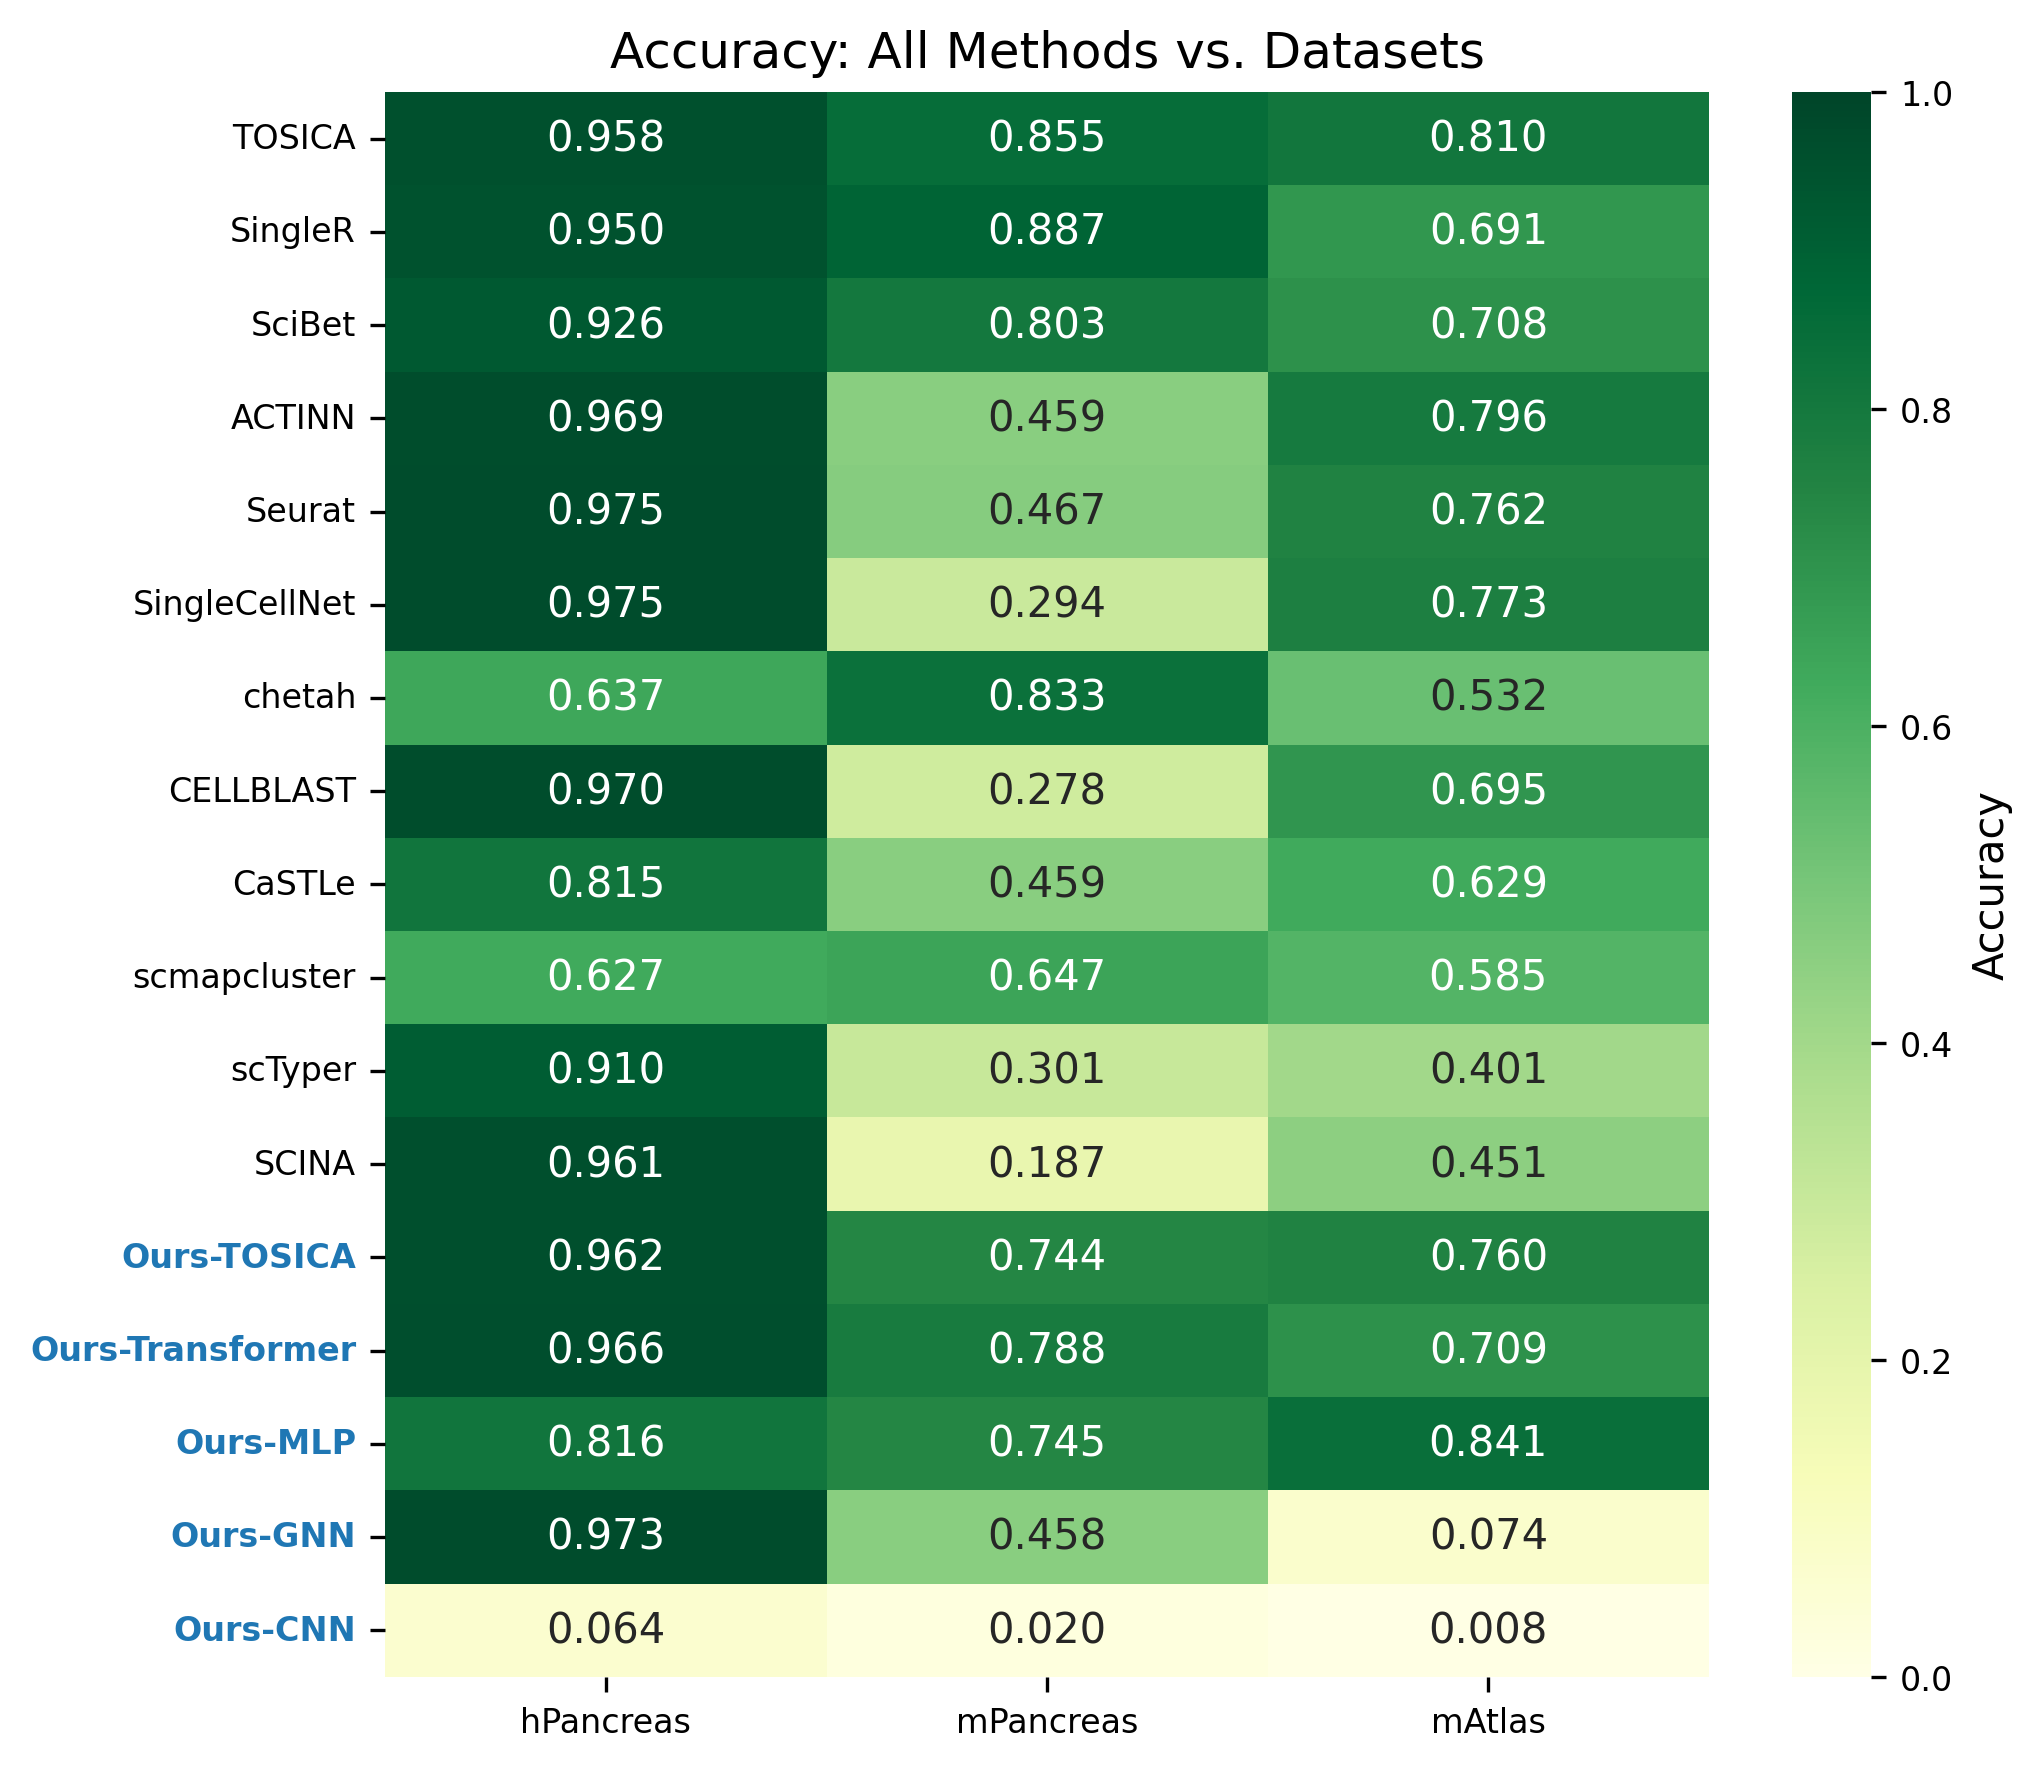
\includegraphics[width=0.7\linewidth]{figures/fig_leaderboard.png}
    \caption{Accuracy heatmap across methods and datasets. Our models (bold
    blue) are compared against 19 published baselines. Rankings shift
    substantially between datasets.}
    \label{fig:leaderboard}
\end{figure}

\begin{figure}[H]
    \centering
    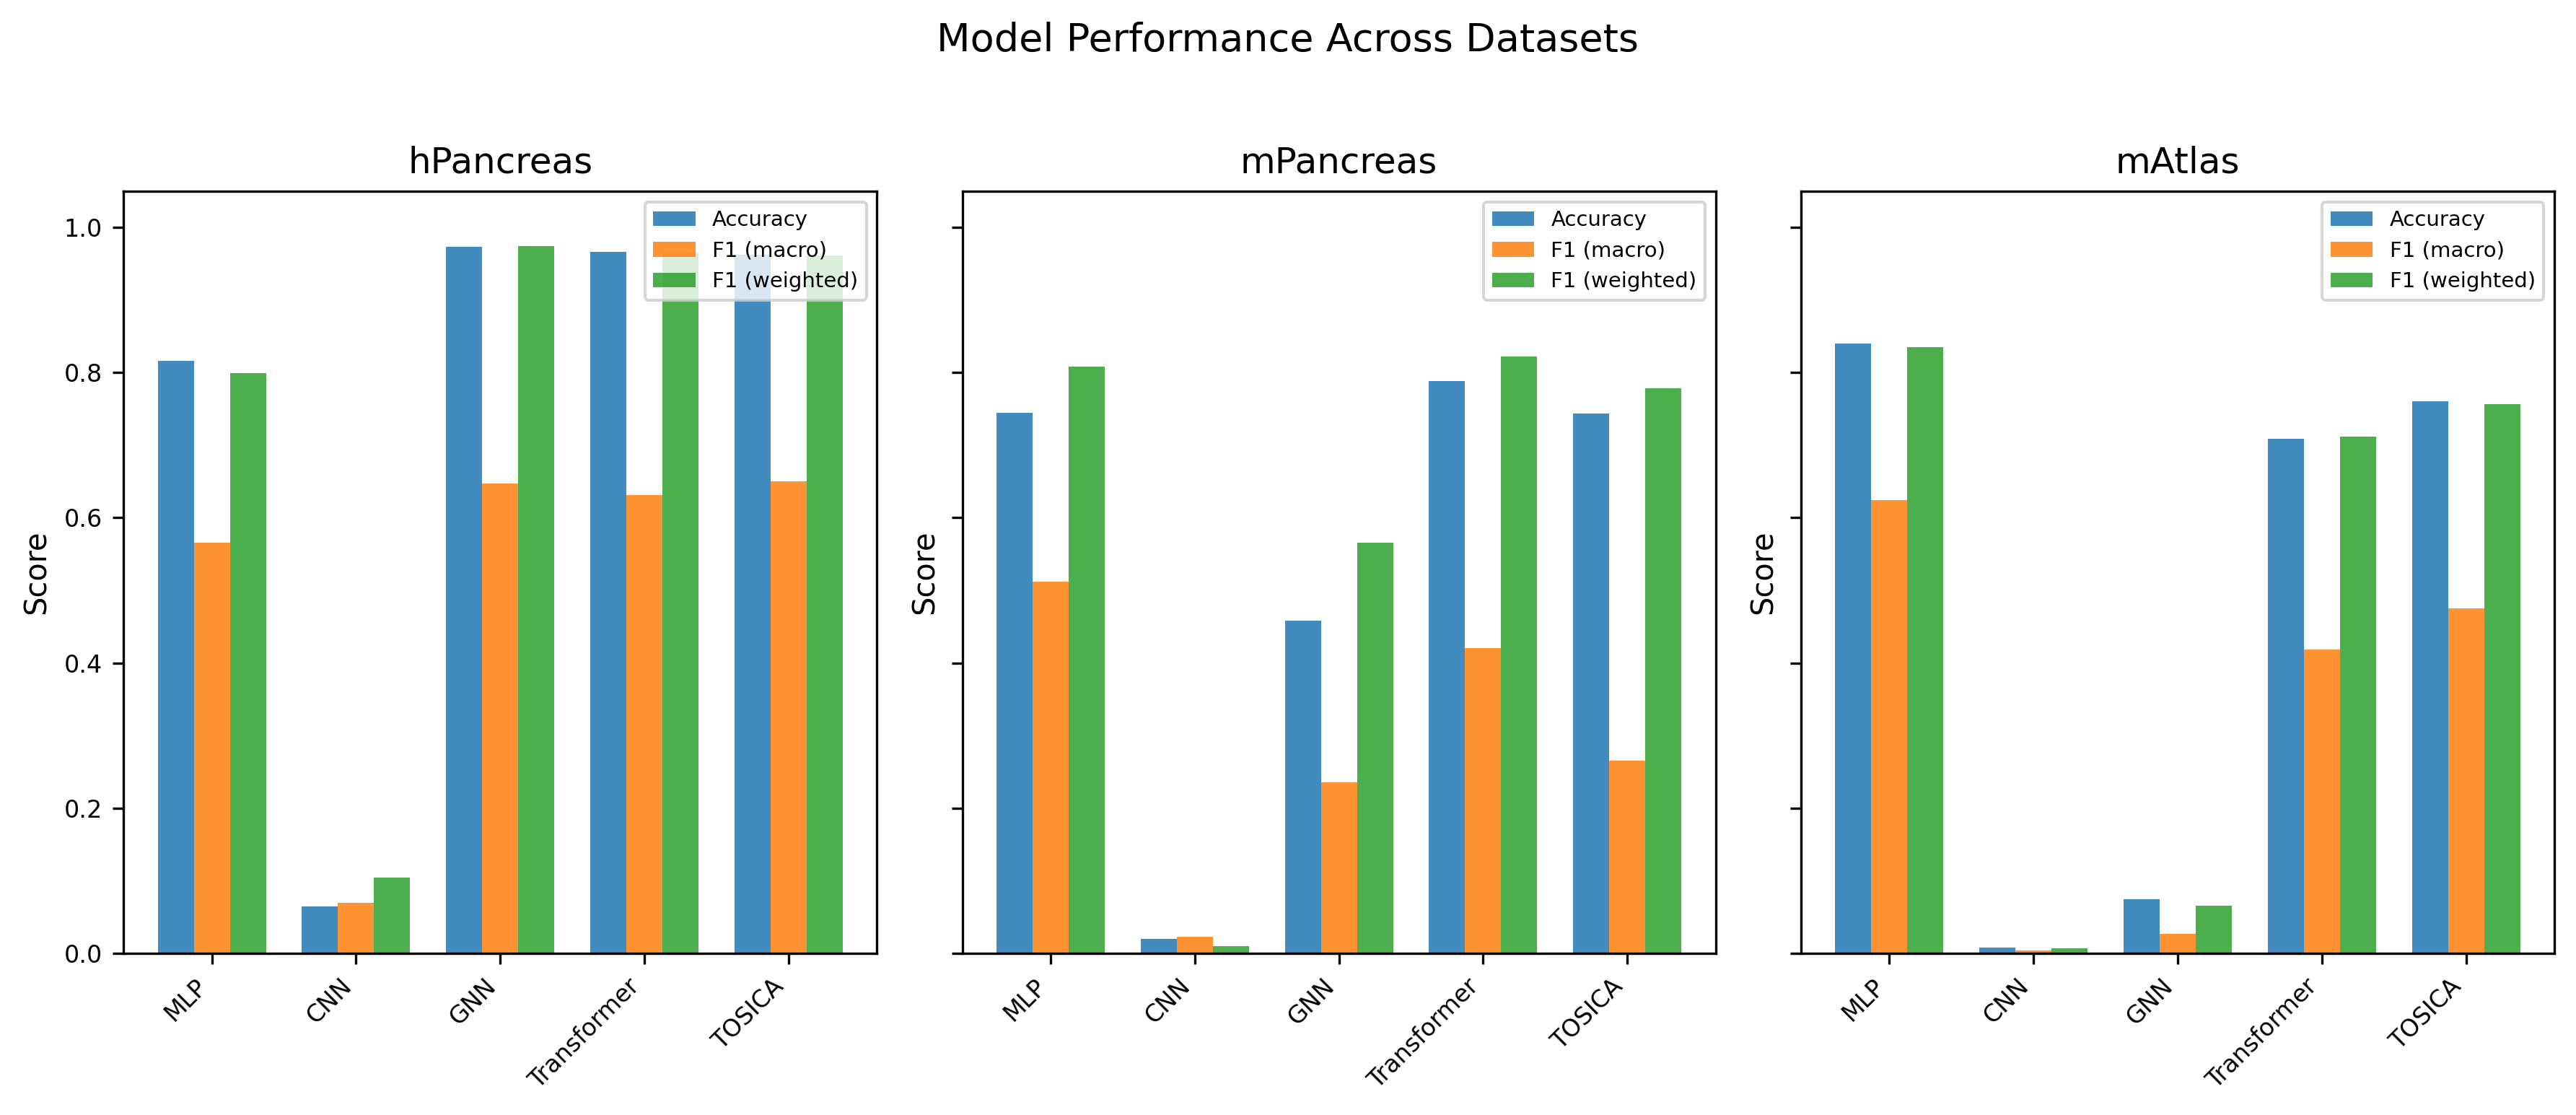
\includegraphics[width=\linewidth]{figures/fig_model_comparison.png}
    \caption{Per-dataset comparison of our five models on accuracy, macro F1,
    and weighted F1. The MLP shows high macro F1 on mPancreas despite lower
    accuracy, indicating better per-class balance than the Transformer.}
    \label{fig:comparison}
\end{figure}

\subsection{CNN Limitations on Gene Expression}
The CNN consistently fails across both datasets (6.5\% and 21.8\% accuracy).
Gene expression vectors lack the spatial locality that makes 1D convolutions
effective on sequential data. Gene ordering is arbitrary, so learned
convolutional filters have no consistent spatial patterns to exploit.

\subsection{TOSICA vs.\ Transformer Gap}
Our Transformer matches or slightly exceeds the external TOSICA library on
both datasets, despite sharing the same core architecture. The gap reflects our
improved data pipeline: consistent HVG selection, balanced oversampling, and
species-appropriate Reactome GMT files. This confirms that preprocessing and
implementation choices can matter as much as architectural novelty.

\subsection{Challenges of Benchmark Reproducibility}
Of the six original TOSICA benchmark datasets, only three could be exactly
reproduced. The discrepancies in hArtery, hBone, and mBrain highlight a broader
issue in computational biology: published benchmarks often rely on implicit
filtering steps, version-specific annotations, or preprocessing details not
fully documented in methods sections. Standardized, versioned benchmark
distributions would substantially improve reproducibility.

% ══════════════════════════════════════════════════════════════════════════════
\section{Conclusion}

We benchmarked five deep learning architectures (MLP, CNN, GNN, Transformer,
TOSICA) on three TOSICA benchmark datasets, comparing against 19 published cell
type annotation methods. On hPancreas, our GNN ranks 3rd out of 24 methods
(97.30\%). On mPancreas, the Transformer leads at 78.92\%. On mAtlas (120
classes), our MLP ranks 1st out of 21 methods (84.05\%), surpassing all
published baselines.

Key findings:
\begin{enumerate}
    \item Model rankings depend strongly on dataset structure---GNNs excel
    when cell similarity is preserved across splits (hPancreas); Transformers
    excel on moderate condition shifts (mPancreas); simple MLPs dominate on
    large-scale multi-class problems with sufficient training data (mAtlas).
    \item Implementation details (species-matched GMT, balanced sampling,
    consistent HVG selection) contribute as much to performance as architectural
    choices---our TOSICA re-run and Transformer both exceed published baselines.
    \item Reproducing published benchmarks exactly is challenging; 3 of 6
    datasets could not be validated and were excluded.
    \item The 1D CNN is unsuitable for gene expression classification due to
    the lack of spatial structure in gene ordering.
\end{enumerate}

\bibliographystyle{plainnat}
\begin{thebibliography}{2}
\bibitem{chen2023tosica}
Chen, J., Xu, H., Tao, W. et al.
\newblock Transformer for one stop interpretable cell type annotation.
\newblock \emph{Nature Communications}, 14, 223 (2023).

\bibitem{lin2017focal}
Lin, T.-Y., Goyal, P., Girshick, R., He, K., and Doll\'{a}r, P.
\newblock Focal loss for dense object detection.
\newblock \emph{IEEE ICCV}, 2017.
\end{thebibliography}

\end{document}
